% This file was created by matlab2tikz.
%
%The latest updates can be retrieved from
%  http://www.mathworks.com/matlabcentral/fileexchange/22022-matlab2tikz-matlab2tikz
%where you can also make suggestions and rate matlab2tikz.
%
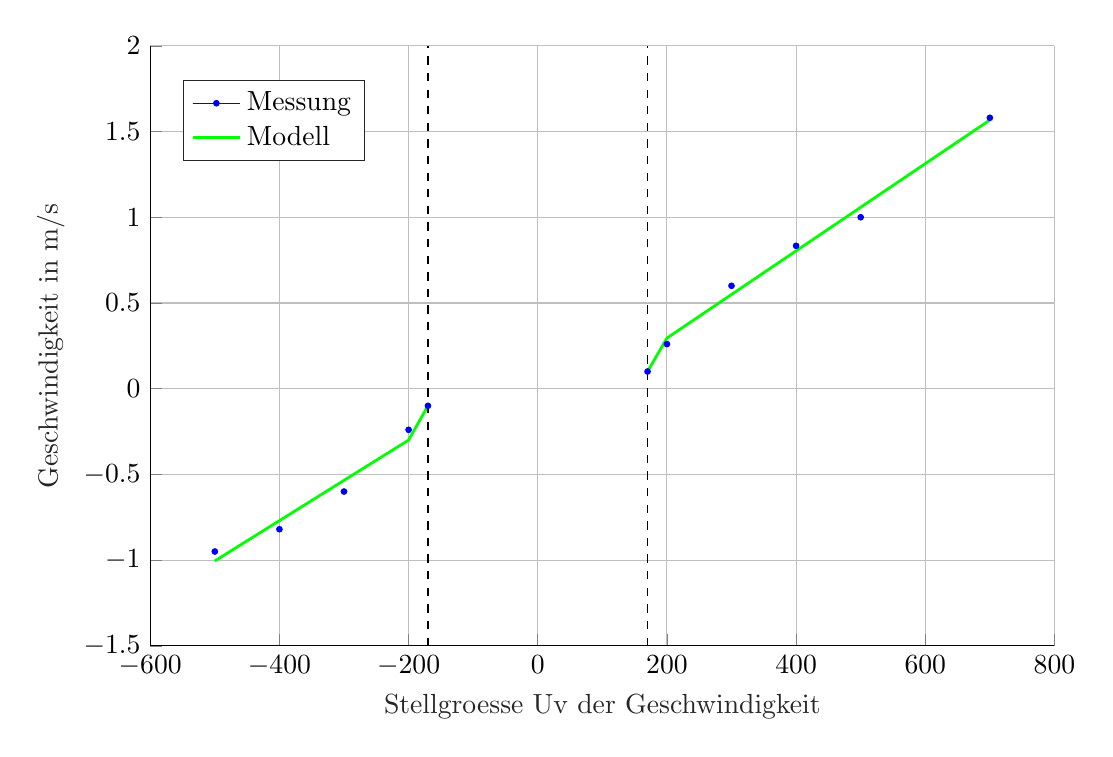
\begin{tikzpicture}

\begin{axis}[%
width=4.521in,
height=3.0in,
at={(0.758in,0.481in)},
scale only axis,
xmin=-600,
xmax=800,
xlabel style={font=\color{white!15!black}},
xlabel={Stellgroesse Uv der Geschwindigkeit},
ymin=-1.5,
ymax=2,
ylabel style={font=\color{white!15!black}},
ylabel={Geschwindigkeit in m/s},
axis background/.style={fill=white},
axis x line*=bottom,
axis y line*=left,
xmajorgrids,
ymajorgrids,
legend style={legend cell align=left, align=left, draw=white!15!black, at={(axis cs:-550,1.8)},anchor=north west}
]

\addplot [color=blue, draw=none, mark=*, mark options={solid, blue}, mark size = 1pt]
  table[row sep=crcr]{%
-500	-0.949999999999989\\
-400	-0.819999999999993\\
-300	-0.600000000000023\\
-200	-0.240000000000009\\
-170	-0.099999999999994\\
170	0.100000000000002\\
200	0.259999999999991\\
300	0.600000000000023\\
400	0.833300000000008\\
500	1\\
700	1.58000000000004\\
};
\addlegendentry{Messung}

\addplot [color=green, solid, line width= 1pt]
  table[row sep=crcr]{%
-500	-1.005\\
-200	-0.300000000000011\\
-170	-0.1\\
};
\addplot [color=green, solid, line width= 1pt, forget plot]
  table[row sep=crcr]{%
170 0.1	\\
200	0.294947297297313\\
700	1.56702162162162\\
};
\addlegendentry{Modell}

\draw [dashed] (-170,-1.5) -- (-170,2);
\draw [dashed] (170,-1.5) -- (170,2);

\end{axis}
\end{tikzpicture}%